\documentclass[a4paper, 10pt]{article}
\usepackage{../../CEDT-Homework-style}

\usepackage{amsmath}
\allowdisplaybreaks

\setlength{\headheight}{14.49998pt}

\begin{document}
\subject[2110203 - Computer Engineering Mathematics II]
\hwtitle{Signal 3}{}{Week 3}{6733172621 Patthadon Phengpinij}{ChatGPT (for\,\LaTeX\,styling and grammar checking)}


% ================================================================================ %
\section{Fourier Series}
% ================================================================================ %



% ================================================================================ %
%                                    Problem 01                                    %
% ================================================================================ %
\begin{problem}
Find the Fourier series of the following periodic function:

\begin{center}
    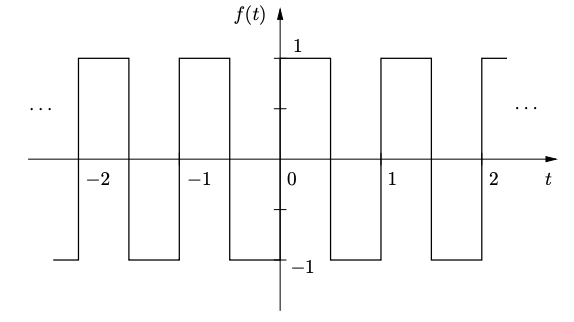
\includegraphics[width=0.6\textwidth]{images/problem_1_reference.png}
\end{center}
\end{problem}

\begin{solution}

\end{solution}
% ================================================================================ %

\newpage

% ================================================================================ %
%                                    Problem 02                                    %
% ================================================================================ %
\begin{problem}
Find the Fourier Series (FS) of the periodic function \( x(t) \) which are provided as follows.
\end{problem}


% === Problem 2.1. === %
\begin{subproblems}[start=1]
    \item \( x(t) = \frac{\pi t^3}{2};\; -1 < t < 1 \)
\end{subproblems}

\begin{solution}

\end{solution}
% ==================== %

\newpage 

% === Problem 2.2. === %
\begin{tosubmit}
\begin{subproblems}[start=2]
    \item \( x(t) = \pi - t;\; -\pi \leq t \leq \pi \)
\end{subproblems}

\par\noindent\submitsolution

\end{tosubmit}
% ==================== %

\newpage

% === Problem 2.3. === %
\begin{tosubmit}
\begin{subproblems}[start=3]
    \item \( x(t) = t^2 + \sin^3(\pi t);\; -1 \leq t \leq 1 \)
\end{subproblems}

\par\noindent\submitsolution

\end{tosubmit}
% ==================== %
% ================================================================================ %


\end{document}